\documentclass{beamer}
\mode<presentation> {
\usetheme{Madrid}
}
%\usepackage{beamerthemeshadow}
\usepackage[utf8]{inputenc}
%\usepackage[latin1]{inputenc}
\usepackage[T1]{fontenc}
\usepackage[brazil]{babel}
\usepackage{graphics,amssymb,amsfonts,amsmath}
\usepackage{tikz}
\usepackage{enumerate,hyperref}
\usepackage{palatino}	% Fonte sem serifa
\usepackage{ragged2e}	% Paragrafo justificado
\usepackage{minted}	% Highlight para codigos de programacao
\usepackage{booktabs} % tabelas
\usepackage{caption}
\usepackage{algorithm,algorithmic}
\usepackage[scientific-notation=true]{siunitx}
\sisetup{round-precision=4,round-mode=figures,scientific-notation=true}


\usepackage{lipsum}
\newcommand\Fontvi{\fontsize{6}{7.2}\selectfont}


% Tela cheia
%\hypersetup{pdfpagemode=FullScreen}

% Layout da pagina
\hypersetup{pdfpagelayout=SinglePage}

% Colocando numero de paginas no slide
\setbeamertemplate{footline}[frame number]

% Desativando os botoes de navegacao
\beamertemplatenavigationsymbolsempty



\begin{document}
\title[]{Introdução} % The short title appears at the bottom of every slide, the full title is only on the title page
\author[]{Leandro Bezerra Marinho} % Your name
\institute[IFCE] % (optional, but mostly needed)
{
\textbf{Disciplina: Aprendizagem de Máquina} \\
Programa de Pós-Graduação em Ciência da Computação (PPGCC) \\
Instituto Federal do Ceará (IFCE)
}
\date{\today} % Date, can be changed to a custom date

%\frame{\titlepage} 
\begin{frame}
\titlepage
\end{frame}


\begin{frame}{Resumo}
\tableofcontents
\end{frame}


%================================
\section{Objetivos}
\begin{frame}{Objetivos}
	
	\begin{itemize}
		\item Verificar a aplicação da MLM no reconhecimento de atividades.
		\item Comparar o desempenho da MLM com as redes MLP, ELM e RBF.
		\item Selecionar o conjunto de atributos que contribuam com a tarefa de identificação de atividades.
		\item Analisar a performance da MLM com a distância Euclidiana e Manhattan.
		\item Mostrar uma nova abordagem da MLM baseada nos vizinhos mais próximos.
	\end{itemize}

\end{frame}


%================================
\section{Motivações}
\begin{frame}{Motivações}

	\begin{itemize}
		\item O RAH pode ser usado na segurança, marketing, entretenimento, saúde, entre outros.
		\item Presença de sensores em dispositivos móveis.
		\item Mais acessível e menos intrusivo.
		\item AM permite construir modelos baseados em pouco conhecimento prévio sobre a tarefa de interesse. 
	\end{itemize}
	
\end{frame}

%================================

\section{Aprendizagem de Máquina}
\begin{frame}{Aprendizagem de Máquina}

Mitchell (1997) define AM como:

	\begin{block}{}
	``A capacidade de melhorar o desempenho na realização de alguma tarefa por meio da experiência.''
	\end{block}

\end{frame}

%------------------------------------------------
\subsection{Tipos de Aprendizado}
\begin{frame}{Tipos de Aprendizado}

	\begin{itemize}
		\item \textbf{Supervisionado:} O conjunto de exemplos possui entrada e saída.
		\item \textbf{Não-Supervisionado:} Agrupa-se um conjunto de exemplos não classificados por regularidades.
		\item \textbf{Por reforço:} Dado sucesso ou insucesso global em uma sequência de ações, determina-se qual é a mais desejável em cada situação.
	\end{itemize}
	
\end{frame}

%------------------------------------------------
\subsection{Redes Neurais Artificiais}
\begin{frame}\frametitle{Redes Neurais Artificiais}

\begin{minipage}[0.2\textheight]{\textwidth}
\begin{columns}[T]
	\begin{column}{0.6\textwidth}
		\begin{itemize}
		\item Funcionamento inspirado no neurônio biológico.
		\item Perceptron
			\begin{itemize}
				\item Só resolve problemas linearmente separáveis
			\end{itemize}
		\item MLP, ELM e RBF.
		\end{itemize}
	\end{column}

	\begin{column}{0.4\textwidth}
		\begin{figure}[htpb]
			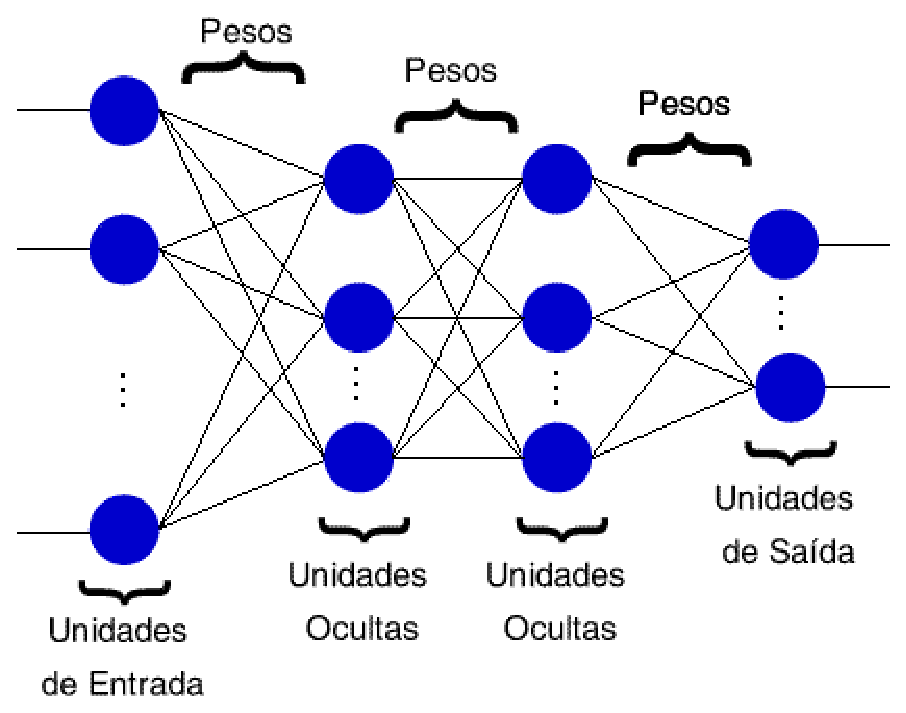
\includegraphics[width=1.0\textwidth]{rna.eps}
			\caption{Modelo de uma Rede Neural Artificial.}
		\end{figure}  
	\end{column}
\end{columns}
\end{minipage}

\end{frame}

%------------------------------------------------

\subsubsection{MLP}
\begin{frame}\frametitle{MLP (Perceptron de Múltiplas Camadas)}
	\begin{itemize}
		\item Pode ter uma ou mais camadas intermediárias.
		\item A entrada da função de ativação é o produto interno dos vetores de entrada.
		\item Algoritmo de treinamento \textit{Backpropagation}
			\begin{itemize}
				\item \textit{Forward}
				\item \textit{Backward}
				\item Foi adotado como condição de parada o número máximo de iterações.
			\end{itemize}
		\item Separa padrões de entrada com hiperplanos.
		\item Foi utilizada a tangente hiperbólica como função de ativação.
	\end{itemize}
\end{frame}


%------------------------------------------------

\subsubsection{RBF}
\begin{frame}\frametitle{RBF (Redes de Funções de Base Radial)}
	\begin{itemize}
	    \item Funções de Base Radial
	    	\begin{itemize}
	    		\item Função gaussiana.
	    	\end{itemize}
		\item Possui apenas uma camada oculta.
		\item A entrada da função de ativação é a distancia euclidiana entre os vetores de entrada e de pesos.
		\item Separa padrões de entrada com hiper-elipsóides.
	\end{itemize}
\end{frame}

%------------------------------------------------

\subsubsection{ELM}
\begin{frame}\frametitle{ELM (Máquina de Aprendizado Extrema)}

	\begin{itemize}
		\item Regra simples de aprendizado.
		\item Número de neurônios na camada oculta é maior que a dimensão do vetor de entrada.
		\item Pesos da camada oculta são gerados aleatoriamente.
		\item Pesos da camada de saída são ajustados para minimizar o EQM.
		\item Foi utilizado a tangente hiperbólica como função de ativação.
	\end{itemize}
	
\end{frame}


%================================
\section{MLM}

\begin{frame}{MLM}

	\begin{itemize}
		\item[] Mapeamento entre configurações geométricas dos pontos no espaço de entrada e saída.
	\end{itemize}

	\begin{itemize}
		\item Formulação
		\item Regressão entre Distâncias
		\item Estimativa da saída
		\item Algoritmos de Treinamento e Teste
		\item MLM-NN
	\end{itemize}

\end{frame}

%------------------------------------------------
\begin{frame}{Formulação}

Dado $N$ pontos de entrada $\mathbf{X} $ e as saídas correspondes $\mathbf{Y} $, queremos estimar $\mathrm{f}$ a partir dos dados com o modelo.
\begin{equation*}
%
\mathbf{Y} = \mathrm{f}(\mathbf{X}) + \mathbf{R}.
%
\end{equation*}
onde $\mathbf{R} $ é a matriz de resíduos.

%Precisa-se reconstruir o mapeamento entre as matrizes de distância de entrada $ \mathbf{D}_x $ e as correspondentes matrizes de distância de saída $ \boldsymbol{\Delta}_y $.

\end{frame}

%------------------------------------------------
\begin{frame}{Regressão entre Distâncias}

	\begin{itemize}
		\item Para uma seleção de $K$ pontos de referência dos dados de entrada e suas respectivas saídas.
		\item $ \mathbf{D}_x \in \mathbb{R}^{N \times K} $ contêm as distâncias entre os $N$ pontos de entrada e os $K$ pontos de referência.
		\item $\boldsymbol{\Delta}_y \in \mathbb{R}^{N \times K} $ contém as distâncias entre os $N$ pontos de saída e as saídas dos $K$ pontos de referência.
		\item O modelo para estimar $\mathrm{g} $ é portanto
			\begin{itemize}[]
				\item[] $\boldsymbol{\Delta}_y = \mathrm{g}(\mathbf{D}_x) + \mathbf{E},$
				\item[] onde $\mathbf{E} $ é a matriz de resíduos.
			\end{itemize}
	\end{itemize}
	
%\begin{equation*}
%%
%\boldsymbol{\Delta}_y = \mathrm{g}(\mathbf{D}_x) + \mathbf{E},
%%
%\end{equation*}

\end{frame}

%------------------------------------------------

\begin{frame}{Regressão entre Distâncias}

	\begin{itemize}
		\item Assumindo que $\mathrm{g} $ é linear, o modelo torna-se
			\begin{itemize}[]
				\item[] $ \boldsymbol{\Delta}_y = \mathbf{D}_x \mathbf{B} + \mathbf{E}. $
				\item[] As colunas da matriz $\mathbf{B}$ correspondem aos coeficientes para as $K$ respostas.
			\end{itemize}
		\item A matriz  $\mathbf{B}$ pode ser estimada através do método dos mínimos quadrados:
			\begin{itemize}[]
				\item[] $ \mathbf{\widehat{B}} = (\mathbf{D}_{x}^{\intercal}\mathbf{D}_x)^{-1}\mathbf{D}_{x}^{\intercal}\boldsymbol{\Delta}_y. $
			\end{itemize}
	\end{itemize}

\end{frame}

%------------------------------------------------

\begin{frame}{Regressão entre Distâncias}
	\begin{itemize}
	    \item Dado um ponto de teste $\mathbf{x}$ e o vetor de distância  $\mathbf{d}(\mathbf{x}, \mathcal{R})$ entre este ponto e os $K$ pontos de referência.
	    \item As distâncias correspondentes entre a saída desconhecida $\mathbf{y}$ e as saídas conhecidas dos pontos referências são estimadas por
	    \begin{itemize}[]
	    	\item[] $\boldsymbol{\widehat{\delta}}(\mathbf{y}, \mathcal{T}) = \mathbf{d}(\mathbf{x}, \mathcal{R})\mathbf{ \widehat{B}}$
	    \end{itemize}
	\end{itemize}
\end{frame}

%------------------------------------------------

\begin{frame}{Regressão entre Distâncias}

\begin{minipage}[0.2\textheight]{\textwidth}
	\begin{columns}[T]
	\begin{column}{0.6\textwidth}
		\begin{itemize}
			\item O vetor $ \boldsymbol{\widehat{\delta}}(\mathbf{y}, \mathcal{T}) $ fornece uma estimativa da configuração geométrica entre $ \mathbf{y} $ e o conjunto de pontos de referência $ \mathcal{T} $.
		\end{itemize}
	\end{column}
	
	\begin{column}{0.4\textwidth}
		\begin{figure}[!ht]
		\centering
		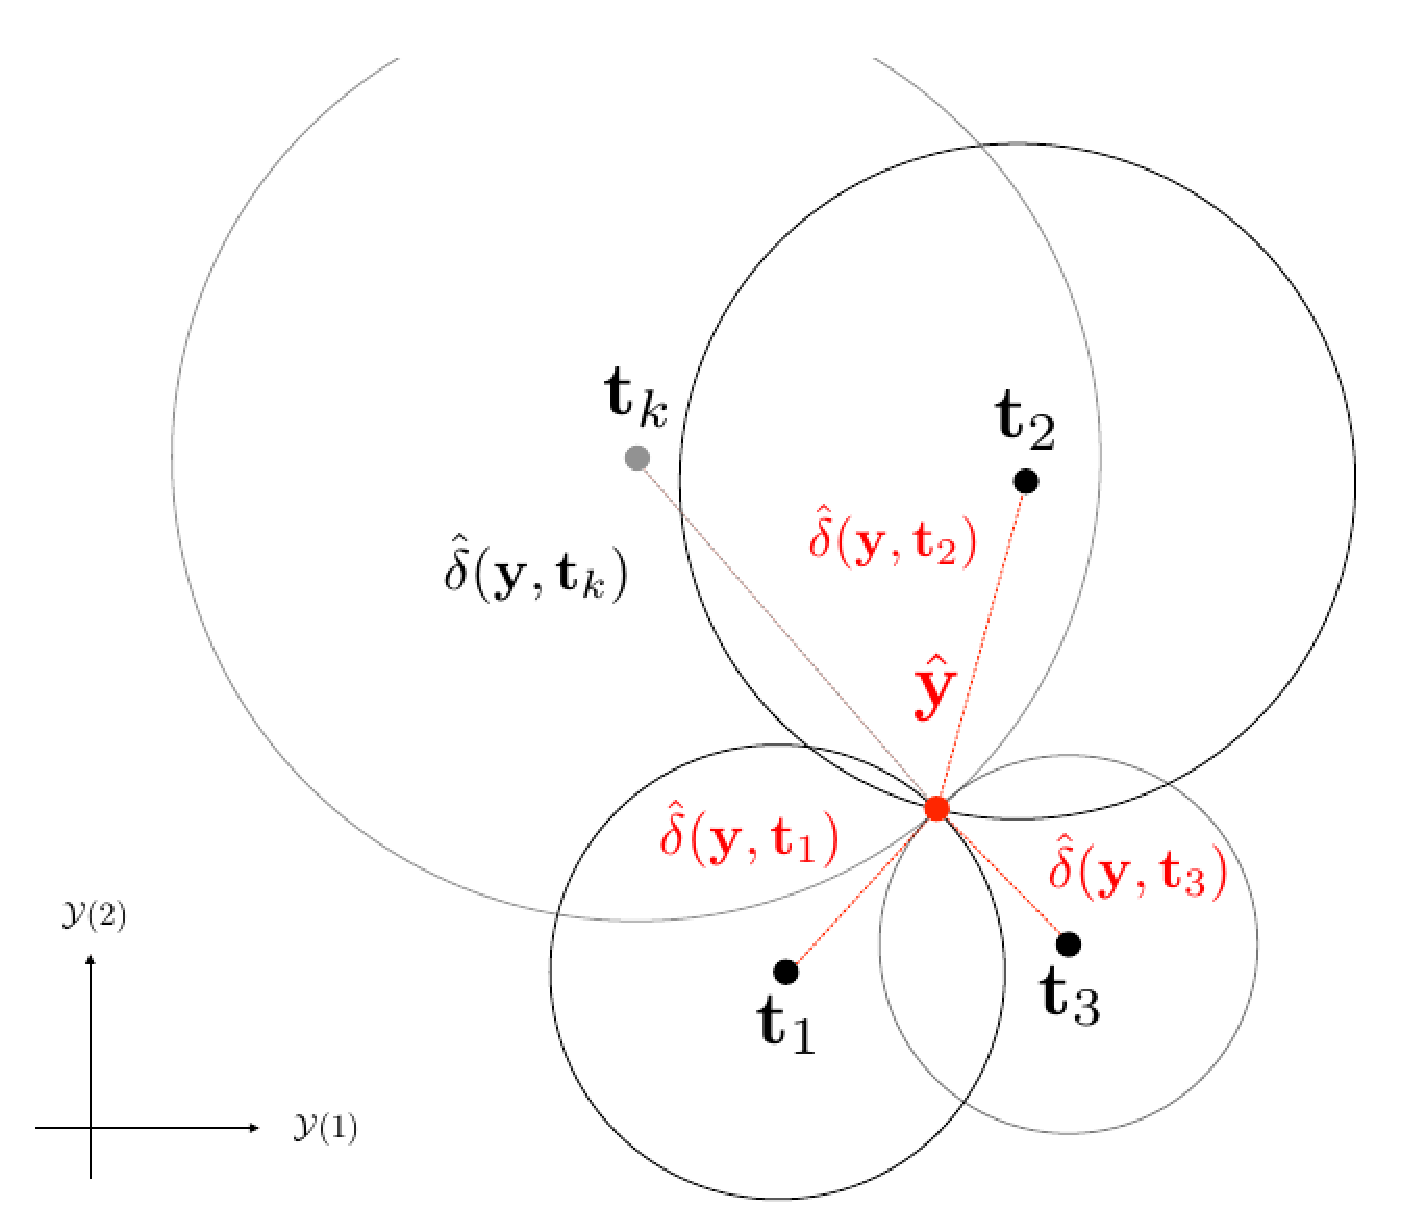
\includegraphics[width=45mm,scale=.35]{output_estimation.eps}
		\caption{Procedimento para obter estimativa}
		\end{figure}	\end{column}
	\end{columns}
	
\end{minipage}

\end{frame}

%------------------------------------------------

\begin{frame}{Estimativa da saída}

	\begin{itemize}
	    \item A estimava da saída $\mathbf{y}$ pode ser formulado como um problema de otimização.
	    \item A solução pode ser alcançada usando o método gradiente descendente ou o algoritmo Levenberg-Marquardt sobre a equação:
	    	\begin{itemize}
	    		\item $\mathbf{ \widehat{y} }= \underset{y}{\arg\min}\sum_{k=1}^{K}((\mathbf{y} - \mathbf{t}_k)^{'}(\mathbf{y} - \mathbf{t}_k) - \widehat{\delta}^{2}(\mathbf{y}, \mathbf{t}_k))^{2}.$ (1)
	    	\end{itemize}
	 \end{itemize}

\end{frame}


%------------------------------------------------

\begin{frame}{Algoritmo de Treinamento da MLM}

	\begin{algorithm}[H]
	\caption{Algoritmo de Treinamento da MLM}
	\begin{algorithmic}[1]
	\REQUIRE Conjunto de treinamento $\mathcal{X}$, $\mathcal{Y}$ e $K$.%
	\ENSURE $ \mathbf{ \widehat{B} }$, $ \mathcal{R} $ e $ \mathcal{T} $.%
	\STATE Aleatoriamente selecione $K$ pontos de referência, $\mathcal{R}$, de $\mathcal{X}$ e suas saídas correspondentes, $\mathcal{T}$, de $\mathcal{Y}$;%
	\STATE Calcule $\mathbf{D}_x$: A matriz de distância entre $\mathcal{X}$ e $\mathcal{R}$;%
	\STATE Calcule $\boldsymbol{\Delta}_y$: A matriz de distância entre $\mathcal{Y}$ e $ \mathcal{T}$;%
	\STATE Calcule $\mathbf{\widehat{B}} = (\mathbf{D}_x^{\intercal}\mathbf{D}_x)^{-1}\mathbf{D}^{\intercal}_x\boldsymbol{\Delta}_y $;%
	\end{algorithmic}
	\end{algorithm}

\end{frame}


%------------------------------------------------
\begin{frame}{Algoritmo de Teste da MLM}

	\begin{algorithm}[H]
	\caption{Algoritmo de Teste da MLM}\label{Alg:MLM_teste}
	\begin{algorithmic}[1]
	\REQUIRE $ \mathbf{ \widehat{B}}, \mathcal{R}, \mathcal{T}$ e $\mathbf{x}$.%
	\ENSURE $\mathbf{ \widehat{y} }$.%
	\STATE Calcule $\mathbf{d}(\mathbf{x},\mathcal{R}) $;%
	\STATE Calcule $\boldsymbol{ \widehat{\delta}}(\mathbf{y},\mathcal{T}) = \mathbf{d}(\mathbf{x},\mathcal{R})\mathbf{\widehat{B}}$;%
	\STATE Use $\mathcal{T}$ e $\boldsymbol{\widehat{\delta}}(\mathbf{y},\mathcal{T})$ para encontrar uma estimativa para $\mathbf{y}$. Isto pode ser conseguido pelo algoritmo Levenberg-Marquardt sobre a função custo na equação 1;%
	\end{algorithmic}
	\end{algorithm}

\end{frame}

%\begin{frame}[fragile] % Need to use the fragile option when verbatim is used in the slide
%	\frametitle{Algoritmos de Treinamento e Teste}
%	\begin{example}[Theorem Slide Code]
%	\begin{verbatim}
%	\begin{frame}
%	\frametitle{Theorem}
%	\begin{theorem}[Mass--energy equivalence]
%	$E = mc^2$
%	\end{theorem}
%	\end{frame}\end{verbatim}
%	\end{example}
%\end{frame}

%------------------------------------------------
\subsection{MLM-NN}
\begin{frame}{MLM-NN}

	\begin{itemize}
		\item A estratégia de encontrar a saída através do procedimento de otimização pode ser computacionalmente ``pesada".
		\item \textbf{Nova abordagem:} Estimar a saída $\mathbf{y}$ baseado em $V$ vizinhos mais próximos (\textit{nearest neighbors}).
		\item Uma vez que as distâncias $\hat{\boldsymbol{\delta}}(\mathbf{y}, \mathcal{T})$ tenham sido estimadas, utilizar as classes dos $V$ pontos de referências mais próximos no espaço de saída a $\mathbf{y}$ para escolher a classe do padrão de teste.
			\begin{itemize}
				\item Moda
			\end{itemize}
	\end{itemize}
	
	
%	Nessa abordagem, uma vez que as distâncias $\hat{\boldsymbol{\delta}}(\mathbf{y}, \mathcal{T})$ tenham sido estimadas, pode-se utilizar as classes dos $V$ pontos de referências mais próximos no espaço de saída a $\mathbf{y}$ para estimar a classe do padrão de teste $l$. Dentre as possibilidades, a estratégia de voto majoritário consiste em atribuir a moda das classes dos $V$ vizinhos mais próximos ao padrão de teste. Neste trabalho, a rede MLM com a abordagem dos vizinhos mais próximos será referenciada pela sigla MLM-NN (MLM-Nearest Neighbors). 
	
\end{frame}

%------------------------------------------------

%\begin{frame}\frametitle{Blocks of Highlighted Text}
%	\begin{block}{Block 1}
%	Lorem ipsum dolor sit amet, consectetur adipiscing elit. Integer lectus nisl, ultricies in feugiat rutrum, porttitor sit amet augue. Aliquam ut tortor mauris. Sed volutpat ante purus, quis accumsan dolor.
%	\end{block}
%	
%	\begin{block}{Block 2}
%	Pellentesque sed tellus purus. Class aptent taciti sociosqu ad litora torquent per conubia nostra, per inceptos himenaeos. Vestibulum quis magna at risus dictum tempor eu vitae velit.
%	\end{block}
%	
%\end{frame}

%------------------------------------------------

%\begin{frame}
%	\frametitle{Multiple Columns}
%	\begin{columns}[c] % The "c" option specifies centered vertical alignment while the "t" option is used for top vertical alignment
%	
%	\column{.45\textwidth} % Left column and width
%	\textbf{Heading}
%	\begin{enumerate}
%	\item Statement
%	\item Explanation
%	\item Example
%	\end{enumerate}
%	
%	\column{.5\textwidth} % Right column and width
%	Lorem ipsum dolor sit amet, consectetur adipiscing elit. Integer lectus nisl, ultricies in feugiat rutrum, porttitor sit amet augue. Aliquam ut tortor mauris. Sed volutpat ante purus, quis accumsan dolor.
%
%	\end{columns}
%\end{frame}




%------------------------------------------------
%
%\begin{frame}
%\frametitle{Table}
%\begin{table}
%\begin{tabular}{l l l}
%\toprule
%\textbf{Treatments} & \textbf{Response 1} & \textbf{Response 2}\\
%\midrule
%Treatment 1 & 0.0003262 & 0.562 \\
%Treatment 2 & 0.0015681 & 0.910 \\
%Treatment 3 & 0.0009271 & 0.296 \\
%\bottomrule
%\end{tabular}
%\caption{Table caption}
%\end{table}
%\end{frame}

%------------------------------------------------

%\begin{frame}
%\frametitle{Theorem}
%\begin{theorem}[Mass--energy equivalence]
%$E = mc^2$
%\end{theorem}
%\end{frame}

%------------------------------------------------

%\begin{frame}[fragile] % Need to use the fragile option when verbatim is used in the slide
%\frametitle{Verbatim}
%\begin{example}[Theorem Slide Code]
%\begin{verbatim}
%\begin{frame}
%\frametitle{Theorem}
%\begin{theorem}[Mass--energy equivalence]
%$E = mc^2$
%\end{theorem}
%\end{frame}\end{verbatim}
%\end{example}
%\end{frame}

%------------------------------------------------

%\begin{frame}
%\frametitle{Figure}
%Uncomment the code on this slide to include your own image from the same directory as the template .TeX file.
%%\begin{figure}
%%
\includegraphics[width=0.8\linewidth]{test}
%%\end{figure}
%\end{frame}

%------------------------------------------------

%\begin{frame}[fragile] % Need to use the fragile option when verbatim is used in the slide
%\frametitle{Citation}
%An example of the \verb|\cite| command to cite within the presentation:\\~
%
%This statement requires citation \cite{p1}.
%\end{frame}


%================================
\section{Metodologia}

\subsection{Base de Dados}
\begin{frame}\frametitle{Base de Dados}
	
	\begin{itemize}
		\item Repositório UCI (Reconhecimento de Atividades Humanas Usando Smartphones)%\cite{Anguita:2012}
		\item Utilizou-se sinais tratados do acelerômetro e giroscópio de um \textit{Samsung Galaxy S II}
		\item \textbf{ Treinamento: } 7352 amostras e 561 características.
		\item \textbf{ Teste: } 2947 amostras e 6 classes.
	\end{itemize}

\end{frame}

%------------------------------------------------
\begin{frame}{Modelagem dos Dados para Classificação}

		\begin{table}[h]
		\centering
		\vspace{0.5cm}
		\begin{tabular}{r|l}
	 
		Classe & Representação \\ % Note a separação de col. e a quebra de linhas
		\hline                               % para uma linha horizontal
		Caminhando			& 1 0 0 0 0 0\\
		Subindo Escada	& 0 1 0 0 0 0 \\
		Descendo Escada	& 0 0 1 0 0 0 \\
		Sentado				& 0 0 0 1 0 0 \\	
		Em pé					& 0 0 0 0 1 0 \\
		Deitado				& 0 0 0 0 0 1 \\
	
		\end{tabular}
		\caption{Modelagem das Classes}\label{tab:modelagem_das_classes}
		\end{table}
	
\end{frame}

%================================

\subsection{Experimentos}
\begin{frame}\frametitle{Experimentos}

	\begin{itemize}
		\item Atributos no domínio do tempo, frequência e ambos
		\item \textbf{Validação cruzada:} 10-\textit{folds}
		\item MLP
			\begin{itemize}
				\item \textbf{Taxa de aprendizagem:} 0.1
				\item \textbf{Iterações:} 100
			\end{itemize}
		\item RBF
			\begin{itemize}
				\item \textbf{Gama:} 1, 0.1, 0.01 e 0.001
			\end{itemize}
		\item MLM
			\begin{itemize}
				\item \textbf{Distâncias:} Euclidiana e Manhattan
				\item $K$: ($ 10\%, 20\%, 30\%, \ldots, 90\%, 100\%$) dos dados de treinamento 
			\end{itemize}
		\item MLM-NN
			\begin{itemize}
				\item $K$: ($ 10\%, 20\%, 30\%, \ldots, 90\%, 100\%$) dos dados de treinamento 
				\item \textbf{Vizinhos}: 9, 15 e 25.
			\end{itemize}
	\end{itemize}
	
\end{frame}

%------------------------------------------------
\begin{frame}\frametitle{Experimentos}
Sequência de neurônios da camada oculta para as RNAs.

\begin{table}[h]
	\centering
	\vspace{0.5cm}
	\begin{tabular}{|l|l|}
		\hline
		Métodos & Número de Neurônios \\ \hline \hline
		MLP     & 10 : 50 : 960          \\ \hline
		ELM     & 300 : 50 : 2500          \\ \hline
		RBF     & 10 : 50 : 960          \\ \hline
	\end{tabular}
	\caption{A segunda coluna mostra o ínicio, variação e fim para uma sequência de neurônios.}\label{tab:neur_cc}
\end{table}

Os experimentos foram executados 10 vezes.
\end{frame}

%%------------------------------------------------
%\subsection{Seleção de Atributos}
%\begin{frame}\frametitle{Seleção de Atributos}
%	Os experimentos foram realizados com 
%\end{frame}

%================================
\section{Resultados}
\begin{frame}{Resultados}
%Experimentos com atributos no domínio do tempo.

\begin{table}
\begin{tabular}{l l l}
\toprule
\textbf{Métodos} & \textbf{Média} & \textbf{Desvio Padrão} \\
\midrule
	ELM & 0.9425  & \num{0.0068} \\ \hline
	RBF & 0.9629 & \num{0.0034} \\ \hline
	MLP & 0.9080 & \num{0.0056} \\ \hline
	MLM-E & \textbf{0.9676} & \num{0.0038} \\ \hline
	MLM-M & 0.9528 &  \num{0.0027} \\ \hline
	MLM-NN-9  & 0.9654 &  \num{0} \\ \hline
	MLM-NN-15 & 0.9654 & \num{0} \\ \hline
	MLM-NN-25 & 0.9654 &  \num{0} \\ \hline
\bottomrule
\end{tabular}
\caption{Taxa média de acerto e desvio padrão com atributos no domínio do \textbf{tempo}.}
\end{table}

\end{frame}


%------------------------------------------------
\begin{frame}{Resultados}
\begin{table}
\begin{tabular}{l l l}
\toprule
\textbf{Métodos} & \textbf{Média} & \textbf{Desvio Padrão} \\
\midrule
	ELM & 0.9209 &  \num{0.0026} \\ \hline
	RBF & 0.9532 &  \num{0.0087}  \\ \hline
	MLP & 0.8889 & \num{0.0170} \\ \hline
	MLM-E & \textbf{0.9541} & \num{0.0059}\\ \hline
	MLM-M & 0.9339 & \num{0.0057} \\ \hline
	MLM-NN-9 & 0.9535 &  \num{2.34055564571780e-16} \\ \hline
	MLM-NN-15 & 0.9535 & \num{2.34055564571780e-16} \\ \hline
	MLM-NN-25 & 0.9535 &  \num{2.34055564571780e-16} \\ \hline
\end{tabular}
\caption{Taxa média de acerto e desvio padrão com atributos no domínio da \textbf{frequência}.}\label{tab:result_freq}
\end{table}
\end{frame}


%------------------------------------------------
\begin{frame}{Resultados}
\begin{table}
\begin{tabular}{l l l}
\toprule
\textbf{Métodos} & \textbf{Média} & \textbf{Desvio Padrão} \\
\midrule
	ELM & 0.9369 & \num{0.0075}\\ \hline
	RBF & 0.9658 &  \num{0.0032} \\ \hline
	MLP & 0.9027 &  \num{0.0194} \\ \hline
	MLM-E & 0.9683 &  \num{0.0078} \\ \hline
	MLM-M & 0.9617 & \num{0.0035} \\ \hline
	MLM-NN-9 & \textbf{0.9715} &  \num{1.17027782285890e-16} \\ \hline
	MLM-NN-15 & \textbf{0.9715} & \num{1.17027782285890e-16} \\ \hline
	MLM-NN-25 & \textbf{0.9715} &  \num{1.17027782285890e-16} \\ \hline
\end{tabular}
\caption{Taxa média de acerto e desvio padrão utilizando \textbf{todos os atributos}.}\label{tab:result_todos}
\end{table}
\end{frame}

%------------------------------------------------
\begin{frame}{Resultados}
Taxa média de acerto com atributos no domínio do tempo.
\begin{figure}[h!]
\begin{center}
	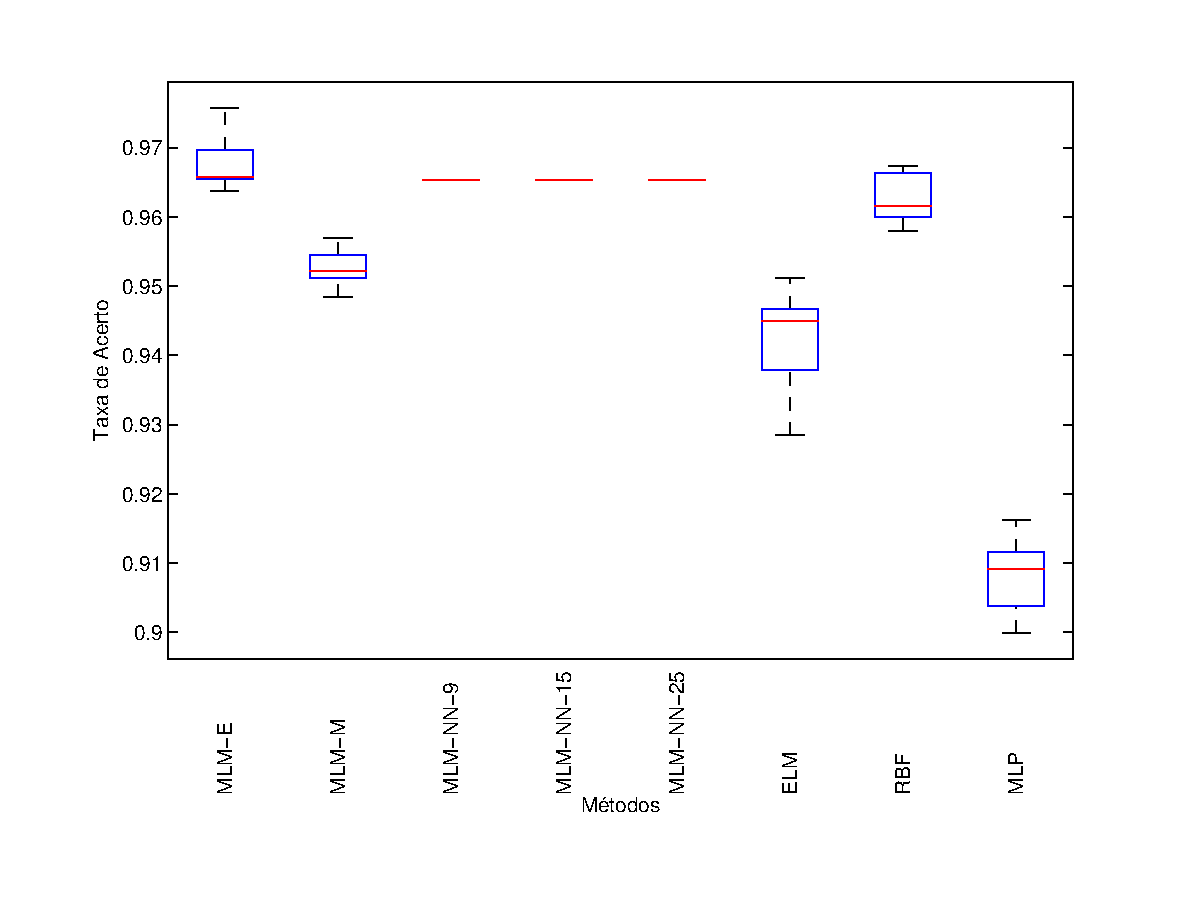
\includegraphics[scale=0.4]{box_temp.eps}
	\caption{Taxa média de acerto com atributos no domínio do \textit{tempo}.}
	\label{img:box_temp}
	\end{center}
\end{figure}

\end{frame}

%------------------------------------------------
\begin{frame}{Resultados}
Taxa média de acerto com atributos no domínio da \textit{frequência}.
\begin{figure}[h!]
\begin{center}
	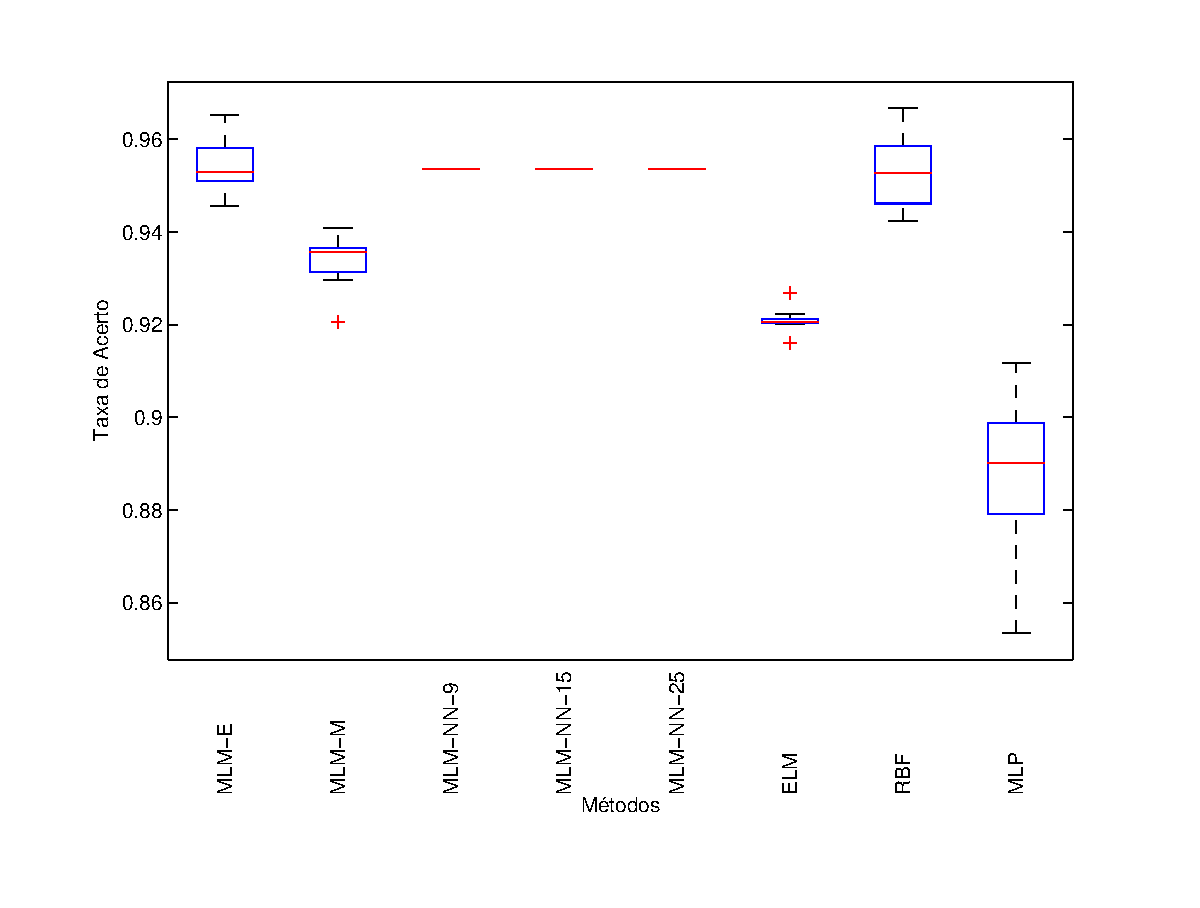
\includegraphics[scale=0.4]{box_freq.eps}
	\caption{Taxa média de acerto com atributos no domínio da frequência.}
	\label{img:box_freq}
	\end{center}
\end{figure}
\end{frame}


%------------------------------------------------
\begin{frame}{Resultados}
Taxa média de acerto com \textit{todos os atributos}.
\begin{figure}[h!]
\begin{center}
	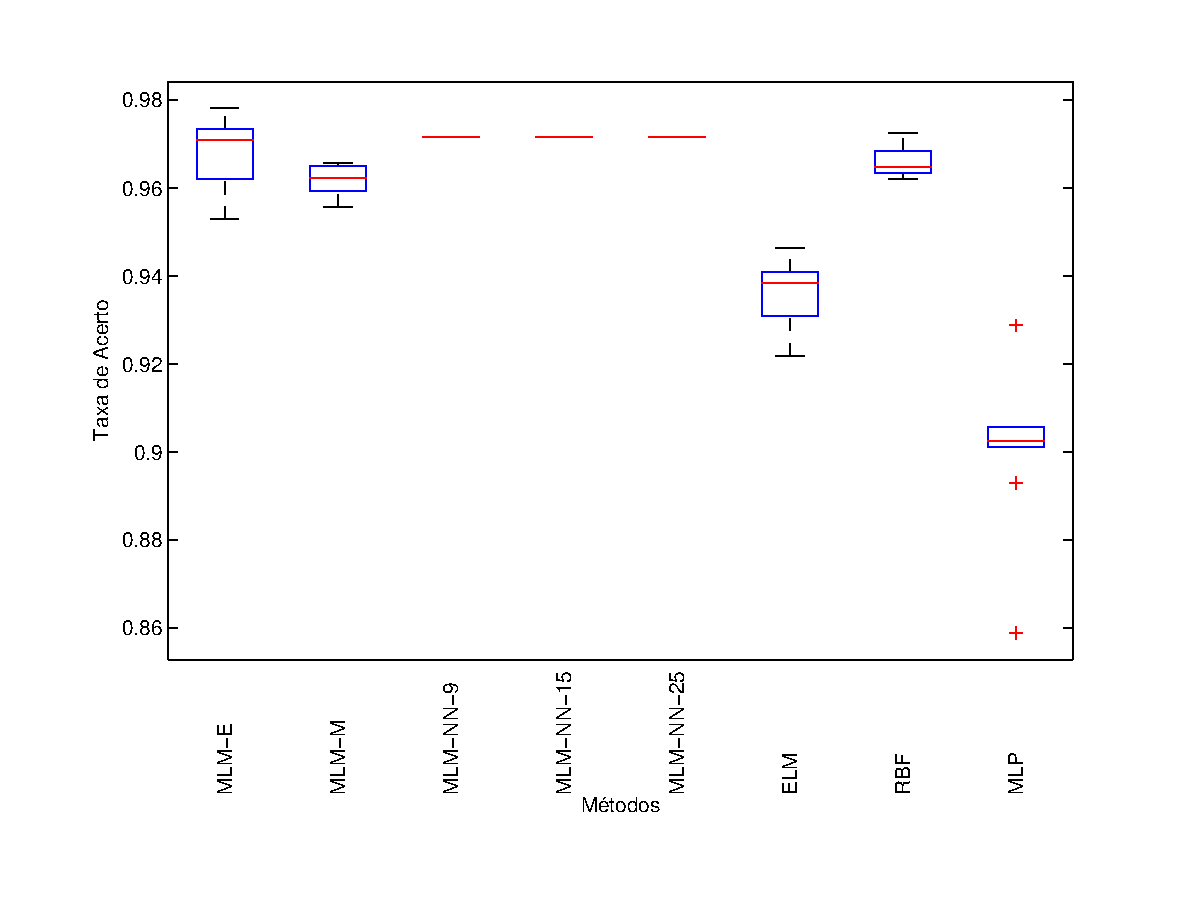
\includegraphics[scale=0.4]{box_tudo.eps}
	\caption{Taxa média de acerto com todos os atributos.}
	\label{img:box_todos}
	\end{center}
\end{figure}
\end{frame}

%================================
\section{Conclusões}
\begin{frame}\frametitle{Conclusões}

\begin{itemize}
		\item Constatou-se que atributos no domínio do tempo foram mais importantes como discriminantes que os correspondentes no domínio da frequência.
		\item No geral, a MLM atingiu as maiores taxas de acerto.
		\item A RBF com seleção aleatória dos centros a partir dos dados, produz resultados bem próximos ou equivalentes aos alcançados pela rede MLM.
		\item Resultados obtidos com o uso da distância Manhatan foram levemente inferiores aos obtidos com distância euclidiana.
		\item A MLM-NN apresentou resultados promissores, principalmente considerando o aumento da velocidade na etapa de teste.
\end{itemize}

\end{frame}



%\begin{frame}\frametitle{Referências Bibliográficas}
%
%\beamertemplatebookbibitems
%  % Start with overview books.
%	\bibitem{gonzales}
%		GONZALEZ, R. C; WOODS, R. E.
%		\newblock {\em  Processamento digital de imagens}.
%		\newblock 3. ed. Pearson Prentice Hall, 2010.
%
%\footnotesize{
%\begin{thebibliography}{99} % Beamer does not support BibTeX so references must be inserted manually as below
%\bibitem[Smith, 2012]{p0} John Smith (2012)
%\newblock Title of the publication
%\newblock \emph{Journal Name} 12(3), 45 -- 678.
%\end{thebibliography}
%}
%
%\begin{thebibliography}
%\bibitem[Mitchell, 1997]{p1} Thomas M. 1997
%\newblock Machine Learning
%\newblock \emph{McGraw-Hill, Inc.}
%\end{thebibliography}
%
%\end{frame}

\appendix
\section<presentation>*{\appendixname}
\subsection<presentation>*{Referências Bibliográficas}

\begin{frame}[allowframebreaks]
  \frametitle<presentation>{Referências Bibliográficas}
    
\begin{thebibliography}{10}
    
  \beamertemplatebookbibitems
  % Start with overview books.		
	\bibitem{braga}
		CARVALHO, Andr\'{e} Carlos, P.L.F. de; BRAGA, Ant\^{o}nio P.; LUDEMIR, T. B.
		\newblock {\em Redes Neurais Artificiais: Teoria e aplicações}
		\newblock LTC Editora, 2007.
		
	\bibitem{cormen}
		CORMEN, Thomas H.; STEIN, Clifford; RIVEST, Ronald L.; LEISERSON, Charles E.
		\newblock {\em Introduction to Algorithms}
		\newblock 3. ed. The MIT Press, 2009.
		
	\bibitem{simon}
		HAYKIN, SIMON S.
		\newblock {\em Redes Neurais: Princípios e Práticas}
		\newblock 2. ed. Bookman Companhia ED, 2002.
		
	\bibitem{mitchell}
		MITCHELL, Thomas M.
		\newblock {\em Machine Learning}
		\newblock 1. ed. McGraw-Hill, 1997.
		
	\bibitem{russel}
		RUSSEL, Stuart; NORVING, Peter.
		\newblock {\em Inteligência Artificial um enfoque Moderno.}
		\newblock 2. ed. Pearson Education, 2004.
		
	\bibitem{valenca}
		VALEN{\c{C}}A, M. J.
		\newblock {\em Fundamentos das Redes Neurais: exemplos em Java}
		\newblock Editora Livro Rápido, 2010.
    
  \beamertemplatearticlebibitems
	\bibitem{allen}
		ALLEN, Felicity R; AMBIKAIRAJAH, Eliathamby; LOVELL, Nigel H; CELLER, B. G.
		\newblock Classification of a known sequence of motions and postures from accelerometry data using adapted gaussian mixture models
		2006.
		
	\bibitem{anguita}
		ANGUITA, Davide; GUIO, Alessandro; ONETO, Luca; PARRA, Xavier; R., Jorge L.
		\newblock Human Activity recognition on smartphones using a multiclass hardware-friendly support vector machine.
		2012.
		
	\bibitem{bao}
		BAO, Ling; INTILLE, Stephen S. 
		\newblock Activity recoginition from user-annotated acceleration data
		2004.
		
	\bibitem{huang}
		HUANG, Guang-Bin; ZHU, Qin-Yu; SIEW, Chee-Kheong.
		\newblock Extreme learning machine: Theory and applications., 
		2003.
		
	\bibitem{huynh}
		HUYNH, Tâm; BLANKE, Ulf; SCHIELE, Bernt.
		\newblock Scalable recognition of daily activities with wearable sensors.,
		2007.
		
	\bibitem{silva}
		SILVA, Vin De; TENENBAUM, Joshua B.
		\newblock Global versus local methods in nonlinear dimensionality reduction.,
		2003.

	\bibitem{amauri}
		SOUZA JUNIOR, A. H.; CORONA, F.; MICHÉ, Y.; LENDASSE, A.; BARRETO, G.; SIMULA, O.
		\newblock Minimal learning machine: A new distance-based method for supervised learning.,
		2013.
		
	\bibitem{tamura}
		TAMURA, Shin'ichi; TATEISHI, Masahiko.
		\newblock Capabilities of a four-layered feedforward neural network: four layers versus three.
		1997.
		
\end{thebibliography}
\end{frame}

%------------------------------------------------



%\section{Section no.1} 
%\frame{\frametitle{Title} 
%Each frame should have a title.
%}
%\subsection{Subsection no.1.1  }
%\frame{ 
%Without title somethink is missing. 
%}


%\section{Section no. 2} 
%\subsection{Lists I}
%\frame{\frametitle{unnumbered lists}
%\begin{itemize}
%\item Introduction to  \LaTeX  
%\item Course 2 
%\item Termpapers and presentations with \LaTeX 
%\item Beamer class
%\end{itemize} 
%}
%
%\frame{\frametitle{lists with pause}
%\begin{itemize}
%\item Introduction to  \LaTeX \pause 
%\item Course 2 \pause 
%\item Termpapers and presentations with \LaTeX \pause 
%\item Beamer class
%\end{itemize} 
%}
%
%\subsection{Lists II}
%\frame{\frametitle{numbered lists}
%\begin{enumerate}
%\item Introduction to  \LaTeX  
%\item Course 2 
%\item Termpapers and presentations with \LaTeX 
%\item Beamer class
%\end{enumerate}
%}
%\frame{\frametitle{numbered lists with pause}
%\begin{enumerate}
%\item Introduction to  \LaTeX \pause 
%\item Course 2 \pause 
%\item Termpapers and presentations with \LaTeX \pause 
%\item Beamer class
%\end{enumerate}
%}

%\section{Section no.3} 
%\subsection{Tables}
%\frame{\frametitle{Tables}
%\begin{tabular}{|c|c|c|}
%\hline
%\textbf{Date} & \textbf{Instructor} & \textbf{Title} \\
%\hline
%WS 04/05 & Sascha Frank & First steps with  \LaTeX  \\
%\hline
%SS 05 & Sascha Frank & \LaTeX \ Course serial \\
%\hline
%\end{tabular}}


%\frame{\frametitle{Tables with pause}
%\begin{tabular}{c c c}
%A & B & C \\ 
%\pause 
%1 & 2 & 3 \\  
%\pause 
%A & B & C \\ 
%\end{tabular} }


%\section{Section no. 4}
%\subsection{blocs}
%\frame{\frametitle{blocs}
%
%	\begin{block}{title of the bloc}
%	bloc text
%	\end{block}
%	
%	\begin{exampleblock}{title of the bloc}
%	bloc text
%	\end{exampleblock}
%	
%	
%	\begin{alertblock}{title of the bloc}
%	bloc text
%	\end{alertblock}
%}

%------------------------------------------------

\begin{frame}\Huge{\centerline{Obrigado pela atenção!}}
\end{frame}

\end{document}

